\chapter{Minimization of Logical Functions}
\addcontentsline{lop}{chapter}{\thechapter \hspace{0.2cm} Minimization of Logical Functions}
\label{chapter:Minimization of Logical Functions}
\graphicspath{ {./chapter03/Fig} }

The intent of this chapter is to explore how to realize 
circuits efficiently.  Efficiency can be measured in
many different ways; number of gates, speed, power
dissipation, and layout size, being just a few. A generally
accepted meaning of minimization is to 
 minimize the number of gates required to realize 
a function in SOP or POS form.  It should be clear that
any logic function can be realized in an SOP or an POS form.
For all but the simplest digital systems, the OR gate cannot 
be eliminated from the SOP realization.  Hence, the focus should 
be on eliminating as many AND gates as possible.
To do this, similar minterms are combined together 
using a trick from Boolean Algebra.

Consider the function $F(A,B,C,D)$ defined by the truth table
below.
$$\begin{array}{c|c|c||c}
A & B & C & F(A,B,C)  \\ \hline
0 & 0 & 0 & 0 \\ \hline
0 & 0 & 1 & 0 \\ \hline
0 & 1 & 0 & 1 \\ \hline
0 & 1 & 1 & 1 \\ \hline
1 & 0 & 0 & 0 \\ \hline
1 & 0 & 1 & 0 \\ \hline
1 & 1 & 0 & 0 \\ \hline
1 & 1 & 1 & 0 \\
\end{array} $$

The canonical SOP expression for this function is $F(A,B,C)=A'BC' + A'BC$.  
This digital circuit requires two NOT gates, two AND gates and one OR gate.  
This realization, however, is not the most minimal one for $F$.  Consider 
the following Boolean Algebra manipulations:

$$\begin{array}{cl}
1 & A'BC' + A'BC = \\
2 & A'B(C' + C) = \\
3 & A'B(1) = \\
4 & A'B
\end{array}$$

This realization of $F$ requires one NOT gate, one AND gate and 
zero OR gates.  Clearly, this realization requires fewer gates then the
first realization.  Hence, it is a more efficient solution.

The minterms used to realize $F(A,B,C)$ are $A'BC'$ and $A'BC$, corresponding 
to the inputs $010$ and $011$ respectively.  The factoring in Line
2 takes advantage of the fact that each of the minterms has two 
variables in common, $A'$ and $B$. This factoring could also be viewed
as a result of the fact that the binary inputs 
of the two minterms have two bits in common $A=0$ and $B=1$ (see 
the truth table for $F$).  The input variable changing between 
the two minterms, $C$, is factored out in Steps 2 and 3 in the above
derivation.  This observation forms the basis of the simplification trick: 


\begin{quote}
\index{trick!simplification}
\textbf{Simplification Trick:} Two minterms whose inputs differ by a single bit 
may be replaced by
a single product term that contains the variables which are the same in 
both minterms and excludes the variable which changes.  
\end{quote}


The simplification trick is used to obtain a simplified form 
for the function $G$ defined by the truth table below.
$$\begin{array}{c|c|c||c}
A & B & C & G(A,B,C)  \\ \hline
0 & 0 & 0 & 0 \\ \hline
0 & 0 & 1 & 1 \\ \hline
0 & 1 & 0 & 1 \\ \hline
0 & 1 & 1 & 0 \\ \hline
1 & 0 & 0 & 0 \\ \hline
1 & 0 & 1 & 1 \\ \hline
1 & 1 & 0 & 1 \\ \hline
1 & 1 & 1 & 0 \\
\end{array} $$


$G$ has four minterms; the main task is to identify which
pairs differ by a single bit.  Inputs 001 and 101 differ by 
a single bit, $A$.  Thus, with the simplification trick,
the product term derived for this pair of minterms is: $B'C$.  
Likewise, the inputs 010 and 110 differ in the $A$ bits, hence
their product term is $BC'$.  Since the product terms are
ORed together in the SOP realization, the reduced product
terms generated by the simplification trick are ORed together,
hence $G(A,B,C)=B'C+BC'$.  Trying to use Boolean Algebra on 
this expression will not produce a more minimal SOP form.

This simplification trick works fine for small examples.
However, when the number of inputs to the function
increases by 1, the number of rows in the truth table
doubles.  Identifying pairs of inputs which differ
by a single bit would quickly become tedious and error-prone.
A more efficient technique requires rearranging the
truth table to make executing the simplification trick easier.

In order to accomplish this goal, the truth table is 
arranged so that rows of the truth table whose inputs differ 
by a single bit are adjacent to one another.  With this 
accomplished, the simplification trick can be invoked by
looking for adjacent 1s.  Such a rearranged truth table
is called a \textit{Karnaugh-map} or Kmap for short.  A
Kmap for a function with three input variables $A,B,C$ is 
shown in the leftmost Kmap.

\begin{figure}
\label{figure:minimiztionThreeVarKmapShell}
\caption{A) The empty shell for a 3-variable kmap.   Note it has
8 empty cells for the output of the function for the corresponding
input. B) The 8 cells of the kmap filled in with the decimal equivalent
of the 3-bit input corresponding to that cell.  Note the bit order is
A as the MSB and C as the LSB.}

$$ \begin{array}{ccc}
	\begin{array} {c||c|c|c|c}
        A \bs BC & 00 & 01 & 11 & 10 \\ \hline \hline
        0        &    &    &    &    \\ \hline
        1        &    &    &    &    \\
	\end{array}$$ 
& &
	\begin{array} {c||c|c|c|c}
        A \bs BC & 00 & 01 & 11 & 10 \\ \hline \hline
        0        & 0  & 1  & 3  & 2  \\ \hline
        1        & 4  & 5  & 7  & 6  \\
	\end{array} \\
A & & B \\
\end{array}
$$

\end{figure}

Each of the cells in the Kmap corresponds to a row of the truth 
table and consequently has a unique combination of $A,B,C$ 
variables.  The $A,B,C$ value of a cell is determined by reading 
off the $A$ bit from the row index on the left and reading the 
$B,C$ bits from the column index at the top.  The Kmap to the 
right has the decimal representation of $ABC$ placed in each
cell.  This numbering of the cells make the placement of 
the 1s of a function easier when specified in the $\sum m$ form.

Most importantly, notice that, given any cell, the cells
to the left, right, up, and down all differ by a single
bit.  For example, the neighbors of the cell for the 
value 5 (``cell 5") are 1, 4, 7, 
each differing from 5 in the $A,C,B$ variable, respectively.
Cells 0 and 3 are not considered neighbors of cell 5 because 
they differ by two bits.  Finally, notice that cell 4 and cell 6 
differ by a single bit $B$, so they should be placed adjacent
to one another, but are separated on the Kmap.  To do this,  
imagine a 3-variable Kmap residing on the surface of a 
torus (doughnut) \index{doughnut}.  The process of manipulating a 
3-variable Kmap onto the surface of a torus is shown in 
Figure~\ref{fig:minimizationTorus}.

\begin{figure}[ht]
\center{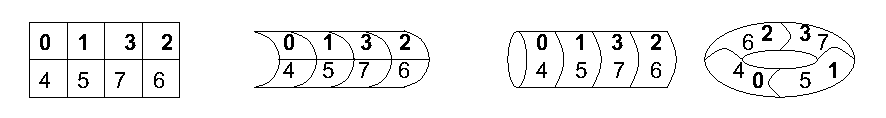
\includegraphics{Torus}}
\caption{The folding and stretching required to transform
a 3-variable Kmap onto the surface of a torus.  The shaded
numbers are on the back side of the surface.}
\label{fig:minimizationTorus}
\end{figure}

When a Kmap is solved correctly the resulting SOP expression
uses the minimum number of gates to realize the circuit 
in SOP form.  Such a minimal SOP expression is referred 
to as a \SOPmin \index{SOP!\SOPmin} expression.

\section{Karnaugh Maps}
Using a Kmap to determine a \SOPmin realization of a function
is a 4-step process. 

\begin{process}{Solving a Kmap}
\label{process:minimizationKmap}

This process is examined by 
determining the \SOPmin expression for the function 
$G(A,B,C)=\sum m(1,2,5,6)$.  Note, this expression is the
same function minimized earlier.  

\textbf{Step 1: Draw an empty kmap}
The first step is to draw an empty Kmap using the input variables of the function $A,B,C$.
Since there are three input variables, this will be a three-variable kmap and 
look exactly like that in Table~\ref{figure:minimiztionThreeVarKmapShell}.
Note that you should draw \textul{all} 3-variable kmaps using this rectangular tabular format with
the variables o the function in question in the upper left corner of the table.
$$ \begin{array} {c||c|c|c|c}
	A \bs BC & 00 & 01 & 11 & 10 \\ \hline \hline
	0        &    &    &    &    \\ \hline
	1        &    &    &    &    \\ 
\end{array} $$


\textbf{Step 2: Place 1s in the Kmap for those inputs for which the function is to equal 1.}
Typically, the 0s of the function are omitted from the Kmap.  It is understood that if
you see a blank space in a Kmap, the function equals 0 for that input.  The Kmap
below shows the Kmap for $G$.

$$ \begin{array} {c||c|c|c|c}
	A \bs BC & 00 & 01 & 11 & 10 \\ \hline \hline
	0        &    & 1  &    & 1  \\ \hline
	1        &    & 1  &    & 1  \\ 
\end{array} $$

\textbf{Step 3: Identify and circle pairs of adjacent 1s in the Kmap}
By adjacent, we mean cells whose inputs differ by a single
bit.  Since these neighbors lie up, down, let and right, we
sometimes call these Manhattan neighbors, because in the
epynomiously named city, streets are laid out in a clean grid 
and blocks consider neighboring when they share a street.
Once you have found a pair of adjacent cells, circle them.
Let's circle the pair of 1's in cell 1 and 5 as well as the pair
of 1's in cell 2 and 6.


$$ \begin{array} {c||c|c|c|c}
	A \bs BC & 00 & 01 & 11 & 10 \\ \hline \hline
\begin{tikzpicture}[overlay]
\draw[red,ultra thick,rounded corners] 		 (1.6,0.3) rectangle (2.2,-0.5);
\draw[blue,ultra thick,rounded corners] 		 (3.1,0.3) rectangle (3.7,-0.5);
\end{tikzpicture}
	0        &    & 1  &    & 1  \\ \hline
	1        &    & 1  &    & 1  \\ 
\end{array} $$


\textbf{Step 4: Write the Boolean expression for the circled cells.}
The Boolean expression for a pair of adjacent 1 is formed by applying
the simplification trick.  Remember that this
technique asks us to write down the input variables which do 
not change and discard the input variable which does change.

For the 1's in the red circle, $B=0$ and $C=1$ for 
both cells and the $A$ variable changes.  Hence, the 
Boolean expression for this grouping is $B'C$.  

For the 1's in the blue circle, $B=1$ and $C=0$ for 
both cells and the $A$ variable changes.  Hence, the 
Boolean expression for this grouping is $BC'$.  


\textbf{Step5: OR together the circled Boolean expressions.}
Since we OR together the minterms when forming a canonical SOP 
expression, it makes sense that we should OR together the product
terms found using the simplification trick.
In our example, this step yields the \SOPmin expression  $G(A,B,C) = B'C + BC'$.
\end{process}

\marginparsep=-1cm
\begin{changemargin}{1.5cm}{1.5cm}

To explore more fully how to solve Kmaps, consider the
following truth table which lists seven functions $F \ldots M$ 
each having three inputs.  The \SOPmin expression is derived 
for each of these functions, along the way 
illustrating many of the properties needed to solve Kmaps.

\begin{tabular}{c|c|c||c|c|c|c|c|c|c|c}
A & B & C & F & G & H & I & J & K & L & M  \\ \hline
0 & 0 & 0 & 0 & 0 & 0 & 1 & 1 & 1 & 1 & 0  \\ \hline
0 & 0 & 1 & 0 & 0 & 1 & 1 & 0 & 1 & 1 & 0  \\ \hline
0 & 1 & 0 & 0 & 1 & 0 & 0 & 1 & 1 & 0 & 0  \\ \hline
0 & 1 & 1 & 1 & 1 & 1 & 0 & 0 & 0 & 1 & 0  \\ \hline
1 & 0 & 0 & 1 & 0 & 0 & 0 & 1 & 0 & 1 & 0  \\ \hline
1 & 0 & 1 & 1 & 0 & 1 & 1 & 1 & 1 & 1 & 0  \\ \hline
1 & 1 & 0 & 0 & 0 & 0 & 0 & 0 & 1 & 0 & 0  \\ \hline
1 & 1 & 1 & 0 & 1 & 1 & 1 & 0 & 1 & 1 & 0  
\end{tabular}

\begin{description}
\item [$F= AB' + A'BC$]
\marginpar{ \tiny $$ \begin{array} {c||c|c|c|c}
        A \bs BC & 00 & 01 & 11 & 10 \\ \hline \hline
        0        &    &    & 1  &    \\ \hline
        1        & 1  & 1  &    &    \\
\end{array} $$ 
\text{Kmap for }F }
The grouping of cell 4 and cell 5 yields the product term $AB'$.  
Cell 5 and cell 3 cannot be combined because they differ in two bits.
What is to do be done with the single cell 3?  Since this cell 
cannot be combined
with another cell, it is just a minterm by itself.  Sad perhaps, 
but perfectly legal.  Hence, $F(A,B,C) = AB' + A'BC$.

\item [$G=A'B + BC$]
\marginpar{ \tiny $$ \begin{array} {c||c|c|c|c}
        A \bs BC & 00 & 01 & 11 & 10 \\ \hline \hline
        0        &    &    & 1  & 1  \\ \hline
        1        &    &    & 1  &    \\
\end{array} $$ 
\text{ Kmap for }G 
\vspace{0.5cm}}

\marginpar{ \tiny $$ \begin{array} {c||c|c|c|c}
        A \bs BC & 00 & 01 & 11 & 10 \\ \hline \hline
        0        &    & 1  & 1  &    \\ \hline
        1        &    & 1  & 1  &    \\
\end{array} $$
\text{ Kmap for }H 
\vspace{0.5cm}}

\marginpar{ \tiny $$ \begin{array} {c||c|c|c|c}
        A \bs BC & 00 & 01 & 11 & 10 \\ \hline \hline
        0        & 1  & 1  &    &    \\ \hline
        1        &    & 1  & 1  &    \\
\end{array} $$ 
\text{ Kmap for }I 
\vspace{0.5cm}}


\marginpar{ \tiny $$ \begin{array} {c||c|c|c|c}
        A \bs BC & 00 & 01 & 11 & 10 \\ \hline \hline
        0        & 1  &    &    & 1  \\ \hline
        1        & 1  & 1  &    &    \\
\end{array} $$ 
\text{ Kmap for }J 
\vspace{0.5cm}}

\marginpar{ \tiny $$ \begin{array} {c||c|c|c|c}
        A \bs BC & 00 & 01 & 11 & 10 \\ \hline \hline
        0        & 1  & 1  &    & 1  \\ \hline
        1        &    & 1  & 1  & 1  \\
\end{array} $$ 
\text{ Kmap for }K 
\vspace{0.5cm}}

\marginpar{ \tiny
$$ \begin{array} {c||c|c|c|c}
        A \bs BC & 00 & 01 & 11 & 10 \\ \hline \hline
        0        & 1  & 1  & 1  &    \\ \hline
        1        & 1  & 1  & 1  &    \\
\end{array} $$ 
\text{ Kmap for }L 
\vspace{0.5cm}}

\marginpar{ \tiny
$$ \begin{array} {c||c|c|c|c}
        A \bs BC & 00 & 01 & 11 & 10 \\ \hline \hline
        0        &    &    &    &    \\ \hline
        1        &    &    &    &    \\
\end{array} $$
\text{ Kmap for }M }

The natural question arising from this Kmap is, ``Can 
cell 3 be reused in two different groups?"  The answer is ``Yes," and the reason
can be demonstrated by performing some Boolean Algebra on the canonical 
SOP expression for $G$.
$$\begin{array}{ll}
G(A,B,C) =	& A'BC' + A'BC + ABC = \\
		& A'BC' + A'BC + A'BC + ABC = \\
		& A'B(C' + C) + BC(A'+A) = \\
		& A'B(1) + BC(1) = \\
		& A'B + BC 
\end{array}$$
In the second line, the minterm $A'BC$ was duplicated using Law 3 of Boolean 
Algebra.  Note, this is the same minterm covered twice in the 
Kmap.  Consequently, if a cell of the Kmap is covered by three different
groupings then it would have to be replicated three times in the Boolean 
Algebra simplification.  

The grouping of cell 2 and cell 3 yields the product term $A'B$.  The 
grouping of cell 3 and cell 7 yield the product term $BC$.  
Consequently, $G(A,B,C) = A'B + BC$.  It is now possible to relate what 
happens in the symbolic expression when $(A,B,C) = (0,1,1)$ to the method
used to solve the Kmap.

\item [$H=C$] 
Grouping can be of size four.  This can be explained by performing Boolean 
Algebra on the canonical SOP expression for $H$.

$$\begin{array}{ll}
H(A,B,C) = 	& A'B'C + A'BC + AB'C + ABC = \\
		& (B+B')A'C + (B'+B)AC =  \\
		& A'C + AC = \\
		& (A'+A)C = \\
		& C 
\end{array}$$
In general, grouping can be of size $2^i \times 2^j$ for integer $i$ and $j$.
It is a common mistake of students to make a grouping of size 3x2 --  3 is not
a power of 2!

\item [$I=A'B'+AC$]
One does not have to form every possible grouping.  It is
a common error for students to include the term $B'C$ in the expression
for $I$.  The expression $B'C'$  does not cause the function to output
an incorrect value. Rather, this expression is not necessary for the
circuit to function properly.  Hence, including the expression $B'C'$ 
would make the circuit larger by one more AND gate than necessary.

\item [$J=A'C'+AB'$] 
Grouping can be made over the edge of the Kmap using the doughnut
\index{doughnut} (torus) property illustrated in Figure~\ref{fig:minimizationTorus}.
Notice, the minterms in the grouping on the upper row 
differ in the $B$ bit.

\item [$K=A'B'+AC+BC'$ or $K=A'C'+B'C+AC$]
A Kmap may have more than one correct solution.

\item [$L=B'+C$]
Avoid the temptation to make a grouping of size $3 \times 2$.
Instead, make two groupings of size $2 \times 2$ which overlap 
in two cells.  Yes, overlapping big groupings is legal, too.



\item [$M=0$] 
This trivial function can be confusing when first encountered.
Notice that regardless of the input, the output of the function 
is always 0.  Hence, $M=0$.
\end{description}
\end{changemargin} 

The process of ``solving" a Kmap correctly leads to a minimal 2-level 
SOP expression (abbreviated \SOPmin).  SOP expressions are composed
of two main levels of gates. A set of AND gates (level 1) leading 
into an OR gate (level 2).  The NOT gates are ignored because they are 
both small and fast compared to AND and OR gates.  The term ``minimal"
refers to the fact that the realization of the function requires 
the fewest possible gates among any 2-level SOP realizations.  

In order to understand how to most efficiently solve a Kmap, some
notation needs to be defined.
An \textit{implicant} \index{Implicant} is a legal grouping of 1s in 
a Kmap.  An implicant which is not contained in any other implicant 
is called a \textit{prime implicant} \index{Implicant!Prime}.  An 
\textit{essential prime implicant} \index{Implicant!Essential Prime} 
is a prime implicant which covers a minterm not covered by any other 
prime implicant. For example, $ABC$ is an implicant in the function 
$L(A,B,C)$, but it is not a prime implicant because it is contained in 
the essential prime implicant $C$.

When solving a Kmap, look for essential prime implicants and 
remove them from consideration.  Removing the 1s from consideration does not
mean removing the 1s from the problem.  If needed, the 1s in an essential
prime implicant can be used to form other groupings.
After the essential prime implicants 
have been removed, look for \textit{secondary essential prime implicants}, 
the essential largest groupings covering the remaining 1s.
 This identification of essential
prime implicants goes on until either all the 1s are covered or 
a situation like the $K$ function results.  The $K$ function has no 
essential prime implicants.  At this point, resort to intuition 
(or brute force search) to minimize the number of groupings
to cover the remaining 1s in the Kmap.  Kmaps can be used to 
minimize functions in a variety of ways.  One such use is discussed below.

\begin{changemargin}{1.5cm}{1.5cm}
Determine the \SOPmin expression for $F(A,B,C) = B'C' + BC' + ABC$.  The
\label{page:SymbToSymb} term \SOPmin implies that a Kmap is 
required to solve the problem. In this case, figure out a way 
determine which region of the Kmap is described by each product term.  
For example, the product term $B'C'$ is equal to 1 when $(B,C) = (0,0)$.
Thus, 1s are placed in cell 0 and cell 4 of the Kmap. The product term $BC'$
results in 1s being placed in cell 2 and cell 6.  The product term $ABC$
requires a 1 to be placed in cell 7.  The resulting Kmap is shown in the 
margin.
\marginpar{\tiny
$$ \begin{array} {c||c|c|c|c}
	A \bs BC & 00 & 01 & 11 & 10 \\ \hline \hline
	0        & 1  &    &    & 1  \\ \hline
	1        & 1  &    & 1  & 1  \\ 
\end{array} $$
}
This Kmap can now be solved to determine the \SOPmin expression;
$F(A,B,C) = C'+AB$.  Incidentally, the grouping of cells 0, 2, 4, 6
in the Kmap above is affectionately referred to as a 
\index{doughnut!Texas} \textit{Texas doughnut} because it has a big 2x2 
grouping straddling the ends of the Kmap.
\end{changemargin}

\section{4-Variable Kmaps}
The Kmap method can be adapted to work with functions of more than three
variables.  These larger Kmaps must be constructed so that adjacent 
cells differ by a single bit in order for the simplification trick 
to work.  For example, a 4-variable Kmap is shown below with the 
decimal equivalent of the binary inputs shown in each cell.

$$ \begin{array} {c||c|c|c|c}
	AB \bs CD & 00 & 01 & 11 & 10 \\ \hline \hline
	00        & 0  & 1  & 3  & 2  \\ \hline
	01        & 4  & 5  & 7  & 6  \\ \hline
	11        & 12 & 13 & 15 & 14 \\ \hline
	10        & 8  & 9  & 11 & 10 \\ 
\end{array} $$

It is easy to verify that adjacent cells differ by a single bit.
In addition, notice that adjacencies run across the top/bottom 
and left/right margins of the Kmap.  In order to better 
understand this new structure, determine the \SOPmin
expressions for the following functions. 

\begin{itemize}
\item $F(A,B,C,D) = \sum m(0,1,4,5,8,9)$
\item $G(A,B,C,D) = \sum m(0,5,7,10,11,14,15)$
\item $H(A,B,C,D) = \sum m(0,2,3,5,6,7,8,10,11,14,15)$
\end{itemize}

\begin{changemargin}{1.5cm}{1.5cm}

\begin{description}
\item [$F=A'C'+B'C'$]  
\marginpar{ \tiny $$ \begin{array} {c||c|c|c|c}
       AB \bs CD & 00 & 01 & 11 & 10 \\ \hline \hline
       00        &  1 &  1 &    &    \\ \hline
       01        &  1 &  1 &    &    \\ \hline
       11        &    &    &    &    \\ \hline
       10        &  1 &  1 &    &    \\
\end{array} $$ 
\text{ Kmap for} F}
Resist the temptation to make a grouping of size $3 \times 2$;
3 is not a power of 2.  Notice, one of the $2 \times 2$
groupings, $B'C'$ spans the edge of the Kmap (Texas doughnut style).


\item [$G=A'B'C'D'+A'BD+AC$] 
\marginpar{ \tiny $$ \begin{array} {c||c|c|c|c}
       AB \bs CD & 00 & 01 & 11 & 10 \\ \hline \hline
       00        &  1 &    &    &    \\ \hline
       01        &    &  1 &  1 &    \\ \hline
       11        &    &    &  1 & 1  \\ \hline
       10        &    &    &  1 & 1  \\
\end{array} $$ 
\text{ Kmap for} G}
This example demonstrates an interesting point: The size of the 
grouping determines the number of variables in the \SOPmin expression.
For example, the grouping for covering one cell, $A'B'C'D'$, has four
variables, the grouping covering two cells, $A'BD$, has three variables 
and the grouping covering four cells, $AC$, has two variables.  The 
larger the grouping, the fewer variables that are required to describe
the grouping, and consequently requires a smaller AND gate.

\item [$H=B'D'+A'BD+C$] 
\marginpar{ \tiny $$ \begin{array} {c||c|c|c|c}
       AB \bs CD & 00 & 01 & 11 & 10 \\ \hline \hline
       00        &  1 &    &  1 &  1 \\ \hline
       01        &    &  1 &  1 &  1 \\ \hline
       11        &    &    &  1 &  1 \\ \hline
       10        &  1 &    &  1 &  1 \\
\end{array} $$ 
\text{ Kmap for} H}
This solution is notable because it contains the 
\textit{HyperDoughnut} \index{Doughnut!Hyper} grouping -- the cells
0,2,8,10 forming the product $B'D'$.  The only other notable 
feature in this Kmap is the large grouping of size 8, $C$.
\end{description}
\end{changemargin}

\section{5-Variable Kmaps}
A 5-variable Kmap is a rearrangement of the rows of a 5-variable
truth table such that adjacent cells of the Kmap differ by a single
input bit.  This rearrangement is accomplished by floating two, 4-variable 
Kmaps one above the other.  A cell in a 5-variable Kmap can be combined with
the cell to its left, right, below, above, up or down!  That is, the three
perpendicular directions along which adjacencies lie must be checked.

Determine the \SOPmin expression for \\
$F(A,B,C,D,E) = \sum m(0,1,2,5,7,8,10,15,16,18,23,24,26,28,29,31)$.
Each of the 4-variable Kmaps is labeled with one of the two possible
values of $A$, 0, or 1.  The decimal values of the inputs can be formed
by converting the binary input $ABCDE$ for each cell into decimal.  The 
4-variable Kmap with $A=0$ is labeled just like an ordinary 4-variable 
Kmap.  The 4-variable Kmap with $A=1$ is labeled in the same order as a 
regular 4-variable Kmap, except the numbering starts at 16 because the MSB
is 1.

$$\begin{array}{cc} 
\begin{array} {c||c|c|c|c}
	BC \bs DE & 00 & 01 & 11 & 10 \\ \hline \hline
	00        & 1  & 1  &    & 1  \\ \hline
	01        &    & 1  & 1  &    \\ \hline
	11        &    &    & 1  &    \\ \hline
	10        & 1  &    &    & 1  \\ 
\end{array}
&
\begin{array} {c||c|c|c|c}
	BC \bs DE & 00 & 01 & 11 & 10 \\ \hline \hline
	00        & 1  &    &    & 1  \\ \hline
	01        &    &    & 1  &    \\ \hline
	11        & 1  & 1  & 1  &    \\ \hline
	10        & 1  &    &    & 1  \\ 
\end{array} \\
A=0 & A=1 \\
\end{array}
$$

This Kmap is notable because it contains the granddaddy of all the
border jumping groupings, the \index{Doughnut!Ultra} \textit{ultra-doughnut}.  
This grouping occupies the eight corners of the 5-variable Kmap.  
A grouping of size four jumps between the two Kmaps.  
Other than this aspect, the solution is fairly straightforward.
$F(A,B,C,D,E)=C'E'+A'B'D'E+CDE+ABCD'$

To conclude the Kmap concept, a few trends 
should be noted.  First, there is a relationship between the
number of variables in a Kmap and the number of neighbors.
\\ \\
\begin{tabular}{l|l}
Variables & Neighbors	\\ \hline
3	  &  3		\\ \hline
4	  &  4		\\ \hline
5	  &  5		\\ 
\end{tabular}
\\ \\
The relationship is linear, that is a cell in a Kmap with 
$N$ variables should have $N$ neighbors.   By considering
the simplification trick, this relationship should make sense. Two cells
are adjacent if their binary representations differ by a single
bit.  An $N$-bit number has $N$ positions where a single bit
could be changed, thus it has $N$ neighbors in the Kmap.  

Also there is a relationship between the number of 1s in a 
grouping and the number of variables appearing in the grouping's
product term.  For example, in the $G(A,B,C,D)$ function
above, the grouping of a single minterm was described by the
product term $A'B'C'D'$ containing four variables.  The largest
grouping of four  minterms was described by the product term
$AC$ containing two variables.  The following table describes 
this relationship for a 5-variable function.
\\ \\
\begin{tabular}{l|l}
Number of 1's	& Variables  \\ \hline
32		&	0	\\ \hline
16		&	1	\\ \hline
8		&	2	\\ \hline
4		&	3	\\ \hline
2		&	4	\\ \hline
1		&	5	\\ 
\end{tabular}
\\ \\
This table demonstrates why making the groupings as large
as possible is desirable, large groupings have smaller AND gates.

\section{Multiple Output Circuits}
In the previous chapter, digital systems with more than one output 
were considered.  Multiple output functions are realized by
realizing each output independently of the others. For example, 
consider a digital system with three inputs $A,B,C$ and two outputs 
$F(A,B,C)$ and $G(A,B,C)$ shown in the truth table below:

$$\begin{array}{c|c|c||c|c}
A & B & C & F & G \\ \hline
0 & 0 & 0 & 0 & 0 \\ \hline
0 & 0 & 1 & 0 & 0 \\ \hline
0 & 1 & 0 & 0 & 1 \\ \hline
0 & 1 & 1 & 1 & 1 \\ \hline
1 & 0 & 0 & 1 & 0 \\ \hline
1 & 0 & 1 & 1 & 0 \\ \hline
1 & 1 & 0 & 0 & 0 \\ \hline
1 & 1 & 1 & 0 & 1 \\
\end{array}$$

\begin{changemargin}{1.5cm}{1.5cm}
If the functions are solved independently of one another,
$F(A,B,C)=AB'+A'BC$ and $G(A,B,C) = BC + A'BC'$.  The only
connection the two circuits have to each other is their inputs, both
share the same $(A,B,C)$.  Thus, when $(A,B,C) = (1,0,1)$ 
$F=1$ and $G=0$ just as expected according to
the truth table.  The circuit diagram of the $F$ and $G$ 
functions is shown in Figure~\ref{fig:minimizationMultiOut}.

\marginpar{ \tiny
$$ \begin{array} {c||c|c|c|c}
        A \bs BC & 00 & 01 & 11 & 10 \\ \hline \hline
        0        &    &    & 1  &    \\ \hline
        1        & 1  & 1  &    &    \\
\end{array} $$
$F(A,B,C) = AB' + A'BC$

$$ \begin{array} {c||c|c|c|c}
        A \bs BC & 00 & 01 & 11 & 10 \\ \hline \hline
        0        &    &    & 1  & 1  \\ \hline
        1        &    &    & 1  &    \\
\end{array} $$
$G(A,B,C) = BC + A'BC'$
}
\end{changemargin}

\begin{figure}[ht]
\center{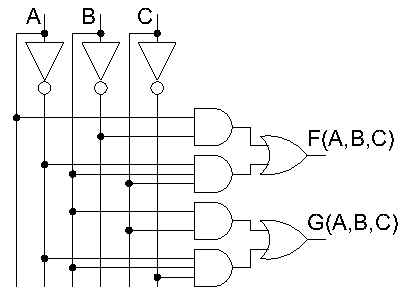
\includegraphics{MultiOut}}
\caption{Two functions, $F$ and $G$, which share inputs.}
\label{fig:minimizationMultiOut}
\end{figure}

\begin{changemargin}{1.5cm}{1.5cm}
However, when you a design circuit that has multiple
outputs which share the same inputs, there are efficiencies
that you can extract if you share product terms.
\index{product term: shared}
  A shared product term is an AND
gate that can be used in the realization of more than one 
function.  For example, consider the two functions 
$H(A,B,C) = \sum m(1,4,5,6)$ and $I(A,B,C) = \sum m(1,2,3,5)$.
\label{page:DualFnc}
\marginpar{ \tiny
$$ \begin{array} {c||c|c|c|c}
        A \bs BC & 00 & 01 & 11 & 10 \\ \hline \hline
        0        &    & 1  &    &    \\ \hline
        1        & 1  & 1  &    & 1  \\
\end{array} $$
$H(A,B,C) = \sum m(1,4,5,6) = B'C + AC'$

$$ \begin{array} {c||c|c|c|c}
        A \bs BC & 00 & 01 & 11 & 10 \\ \hline \hline
        0        &    & 1  & 1  & 1  \\ \hline
        1        &    & 1  &    &    \\
\end{array} $$
$I(A,B,C) = \sum m(1,2,3,5) = B'C + A'B$ 
}

The Kmaps and the solutions for these two functions are shown in 
the margins.  Notice that the grouping $B'C$ appears in both
\SOPmin expressions.  This AND gate need appear only once in the
circuit diagram because its output can be directed to both OR gates 
which form the outputs for $H$ and $I$.  The circuit diagram for 
these two functions is shown in Figure~\ref{fig:minimizationShare}.
\end{changemargin}

\begin{figure}[ht]
\center{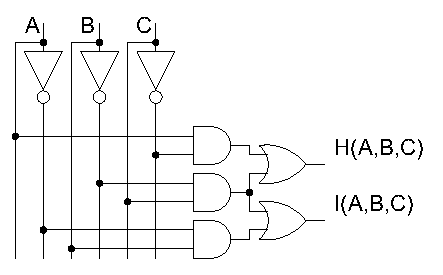
\includegraphics{Share}}
\caption{Two functions which share the product term $B'C$.}
\label{fig:minimizationShare}
\end{figure}

\section{``Don't Cares"}
There are situations when engineers ``don't care" what the output of a
digital system is for certain inputs.  This situation often happens when 
a particular input will never occur.  For example, consider the 
a digital system which classifies its inputs as either even or
odd.  It has four bits of input $a_3 a_2 a_1 a_0$, and one bit 
of output, $F$.  The 4-bit input represents a decimal number, 
$0 \le A \le 9$, the inputs $10 \le A \le 15$ should never be
applied.  The output equals 1 when $A$ is even ( 0 is considered 
an even number) and outputs 0 when $A$ is odd.

\begin{changemargin}{1.5cm}{1.5cm}
As a first attempt to solve this problem, ignore the inputs 
corresponding to $10 \le A \le 15$ and leave the 
corresponding outputs blank.  The outputs are to be defined
for inputs $0 \le A \le 9$. The resulting Kmap and its solution
is shown in the margins.

\marginpar{ \tiny
$$ \begin{array} {c||c|c|c|c}
a_3 a_2 \bs a_1 a_0 & 00 & 01 & 11 & 10 \\ \hline \hline
	00          & 1  &    &    & 1  \\ \hline
	01          & 1  &    &    & 1  \\ \hline
	11          &    &    &    &    \\ \hline
	10          & 1  &    &    &    \\ 
\end{array} $$
$F(a_3,a_2,a_1,a_0)=a_3'a_0'+ a_2'a_1'a_0'$
}

The solution shown in the margin will certainly work correctly,
since the outputs are correctly defined for the legitimate inputs.
However, the realization could have been made more efficient
if the fact that the inputs $10 \le A \le 15$ will never be applied 
had been taken into consideration. Then, it does not matter what the 
circuit outputs when $10 \le A \le 15$.  Notice, that in the first 
solution, implicitly
the illegal inputs were treated as odd numbers; the circuit would
output a 0 for $10 \le A \le 15$. Since these are illegal inputs,
they are assigned any convenient value with an eye on making 
the final realization as
efficient as possible.  To denote this freedom in assigning the
output of the function either value, an ``X" is placed in any 
cell of the Kmap where the output doesn't matter.  These
Xs are referred to as ``don't cares".

The utility of ``don't cares" lies in the fact that they can be 
used to make groupings larger and consequently the realization
of the function more efficient.  If an X can be used to make a 
grouping larger, then it should be included in that grouping.
Including ``don't cares" in a group will cause the circuit to
output 1 for the input corresponding to the ``don't care".  
If, on the other hand,
an X cannot be used in any grouping, then leave it uncovered.
The circuit will output a 0 for the uncovered ``don't care".

To better understand how ``don't cares" are used, they are included
into the even/odd function for inputs $10 \le A \le 15$ and the
resulting Kmap shown in the margin is solved.

\marginpar{ \tiny
$$ \begin{array} {c||c|c|c|c}
a_3 a_2 \bs a_1 a_0 & 00 & 01 & 11 & 10 \\ \hline \hline
	00          & 1  &    &    & 1  \\ \hline
	01          & 1  &    &    & 1  \\ \hline
	11          & X  & X  & X  & X  \\ \hline
	10          & 1  &    & X  & X  \\ 
\end{array} $$
$F(a_3,a_2,2_1,a_0)=a_0'$
}

By using the ``don't cares" in cells 10, 12, and 14, a grouping of
size eight is formed.  This grouping reduces the cost of the solution
to a single inverter.


``Don't cares" are included in the abbreviated canonical SOP form by 
writing a ``$d$" followed by a list of inputs for which the output is
unimportant.  For example, the even/odd function is described 
as $F(A,B,C,D) = \sum m(0,2,4,6,8) + \sum d(10,11,12,13,14,15)$.
\end{changemargin}

``Don't cares" can be used on the input variables of a truth table 
in order to compress the size of the truth table.  Two rows can
be combined when their outputs are the same and their inputs are
adjacent (in the Kmap sense) to one another.  A single ``don't care"
on an input of a row of a truth table generates two rows; one 
with the ``don't care" set to 1 and another with the ``don't care"
set to 0.  For example, the following two truth tables describe 
the same function.

\begin{tabular}{ll}
\begin{tabular}{c|c|c||c}
A & B & C & F(A,B) \\ \hline
x & 0 & x & 0 \\ \hline
x & 1 & 0 & 1 \\ \hline
0 & 1 & 1 & 0 \\ \hline
1 & 1 & 1 & 1 \\ 
\end{tabular} 

&

\begin{tabular}{c|c|c||c}
A & B & C & F(A,B) \\ \hline
0 & 0 & 0 & 0 \\ \hline
0 & 0 & 1 & 0 \\ \hline
0 & 1 & 0 & 1 \\ \hline
0 & 1 & 1 & 0 \\ \hline
1 & 0 & 0 & 0 \\ \hline
1 & 0 & 1 & 0 \\ \hline
1 & 1 & 0 & 1 \\ \hline
1 & 1 & 1 & 1 \\ 

\end{tabular}  \\
Compressed Truth Table & Full Truth Table \\
\end{tabular}

The row $(x,1,0)$ generates two rows in the full truth 
table, $(0,1,0)$ and $(1,1,0)$.  
The row $(A,B,C)=(x,0,x)$ has two ``don't cares".  Since
the values of these ``don't cares" can be selected
independent of one another, this row generates four
rows in the full truth table, $(0,0,0)$, $(0,0,1)$,
$(1,0,0)$, and $(1,0,1)$. In general, a row with $N$ 
``don't cares" generates $2^N$ rows in the full 
truth table.  The motivation for using ``don't cares"
will become more clear in later chapters when digital 
systems with six or more inputs are encountered.

\section{Minimizing to POS}
So far, the chapter has focused on finding efficient 
\SOPmin realizations of circuits.  However, 
Section~\ref{sec:TTtoSymb} provided a function whose POS 
realization was less costly than the SOP realization.
It is not difficult to imagine functions 
for which the \POSmin realization is less costly than 
the \SOPmin realization. In order to derive the 
\POSmin realization of a function $F$, the function
is transformed -- put into a Kmap, a \SOPmin realization
found, and then the \SOPmin realization transformed 
into a \POSmin realization for $F$.  In order for this 
process to work, the two transformations of the function
will have to ``undo" one another so they have no net 
effect on the function.

In order to cover all possibilities, the transform from any of 
the starting forms into one of the ending forms is investigated.

\begin{tabular}{lcr}
$\sum m$   &                    & 	  \\ 
$\prod M$  & $\longrightarrow$  & \SOPmin  \\ 
SOP        &                    & \POSmin \\ 
POS        &                    &     	  \\ \hline
Starting   &                    &  Ending \\ 
Form       &                    &  Form   \\ 
\end{tabular}
\\ \\
Eight potential transforms need to be explored.  For each transformation, a plan is developed;
a series of steps.  The following five helpful facts become the steps in all these plans.

\textbf{Helpful Facts}

\begin{description}
\item [1]
\helpfulStuff{helpful:negateKmap}
Negating a Kmap for $F$ negates $F$.  If all the 
bits in a Kmap for a function $F$ are flipped, then it is
the same as negating the output of $F$.

\item [2] \helpfulStuff{helpful:negateSOP}
Negating a SOP expression for $F$ yields a POS 
\label{page:second} expression for $F'$.  This statement is 
based on Law 9 and Law 9D of Boolean Algebra.  Law 9 states that 
$(x+y)' = x'y'$.  Law 9D states that $(xy)' = x'+y'$.
The transformation from SOP to POS is illustrated
in the following example.

\begin{tabular}[ht]{ll}
$F  = A'B'C' + A'BC + AB' + C$      & negate F \\
$F' = (A'B'C' + A'BC + AB' + C)'$   & Law 9 \\
$F' = (A'B'C')'(A'BC)'(AB')'(C)'$   & Law 9D \\
$F' = (A+B+C)(A+B'+C')(A'+B)(C')$  \\
\end{tabular}

The shortcut typically used to determine the POS expression
is to replace all ANDs and ORs and negate each variable. 

\item [3] \helpfulStuff{helpful:negatePOS}
Negating a POS expression for $F$ yields a SOP 
expression for $F'$.  The proof of this statement is
derived by examining the previous algebraic example from
bottom to top.

\item [4] \helpfulStuff{helpful:prodToSum}
$\sum m(list) = \prod M(list')$.  $list'$ 
denotes the decimal numbers not in $list$.  Since $list$ 
describes those inputs for which the function equals 1, 
$list'$ describes those inputs for which the function 
equals 0. 

\item [5] $F'' = F$.  \helpfulStuff{helpful:doubleNegate}
This expression is just Law 4 of Boolean Algebra.
\end{description}
% 1 \label{helpful:negateKmap}
% 2 \label{helpful:negateSOP}
% 3 \label{helpful:negatePOS}
% 4 \label{helpful:prodToSum}
 % 5 \label{helpful:doubleNegate}

The plans used to transform between forms consist 
of a sequence of steps.  At each step, the function 
(or its complement) is represented in one
of its various forms (Kmap, SOP, $\sum m$, etc..). 
Step 1 always describes the given form of the function.  
Likewise, the last step always describes the desired form
of the function.  The action between the steps is implicit
from the beginning and ending forms.  

To better understand how a plan is put together and how the
transformations are performed, consider a plan for the
transformation of a $\sum m$ expression into a \SOPmin realization.

\begin{process}{Determine \SOPmin given a $\sum m(\ldots)$ expression.}
\label{process:minimizationSumToSOP}
This should be the (by now) familiar process of drawing a kmap 
with the correct number of variable and putting 1's in the cells
where the function equals 1 and then solving the kmap.

\textbf{The Plan:}

\begin{tabular}{|c|c|c|c|}\hline
Step	  & 1  & 2  & 3   \\ \hline
Function  & F  & F  & F \\ \hline
Form	  & $\sum m(\ldots)$ & Kmap & \SOPmin \\ \hline
\end{tabular}
\\ \\
The plan consists of three steps.  The function in all three steps is $F$.   
In Step 1, the function $F$ is written in the $\sum m(\ldots)$
notation.  In the second step, the function is placed into
a Kmap using the process outlined in this chapter. In the 
third step, the \SOPmin expression is derived from the Kmap.
\end{process}

Another familiar transform is handled next.
\begin{process}{Determine  \SOPmin given a SOP expression.}
\label{process:minimizationSOPToSOP}
The only difference in this transformation is the beginning 
form.  The discussion on page~\pageref{page:SymbToSymb} 
illustrates how to put a SOP Boolean expression into a Kmap.  
Once in a Kmap, the remaining steps should be clear.  

\textbf{The Plan:}

\begin{tabular}{|c|c|c|c|}\hline
Step	  & 1  & 2  & 3   \\ \hline
Function  & F  & F  & F \\ \hline
Form	  & SOP & Kmap & \SOPmin \\ \hline
\end{tabular}
\end{process}

The next transformation has a worked out solution to guide
you through the steps of the process.

\begin{process}{Determine \POSmin given a $\sum m(\ldots)$ expression.}
\label{process:minimizationSumToPOS}
\textbf{The Plan:}

\begin{tabular}{|c|c|c|c|c|c|}\hline
Step	  & 1  & 2  & 3  & 4  & 5   \\ \hline
Function  & F  & F  & F' & F' & F''=F \\ \hline
Form	  & $\sum m(\ldots)$ & Kmap & Kmap' & \SOPmin & \POSmin \\ \hline
\end{tabular}
\vspace{0.2cm}

An example shows how this plan is put into practice.
Determine the \POSmin expression for $F(A,B,C) = \sum m(3,4,5)$.

\textbf{Step 1} $F(A,B,C) = \sum m(3,4,5)$.

\textbf{Step 2} The Kmap for $F$ 
$$ \begin{array} {c||c|c|c|c}
        A \bs BC & 00 & 01 & 11 & 10 \\ \hline \hline
        0        &    &    & 1  &    \\ \hline
        1        & 1  & 1  &    &    \\ 
\end{array} $$

\textbf{Step 3} This step relies on helpful fact~\ref{helpful:negateKmap}, 
inverting the entries in a kmap, negates the function.  Thus, the Kmap for $F'$ 
$$ \begin{array} {c||c|c|c|c}
        A \bs BC & 00 & 01 & 11 & 10 \\ \hline \hline
        0        & 1  & 1  &    & 1  \\ \hline
        1        &    &    & 1  & 1  \\ 
\end{array} $$

\textbf{Step 4} Requires that we solve the kmap for F' yielding:
$$F'(A,B,C)= A'B'+AB+BC'$$

\textbf{Step 5} Relies on helpful fact~\ref{helpful:negateSOP},
negating a SOP expression for $F$ yields a POS expression
for $F'$.  We will work through the steps here as a review.

\begin{tabular}[ht]{ll}
$F''(A,B,C) = F(A,B,C)$		& 	$= (A'B'+AB+BC')'$			\\
							&	$= (A'B')'(AB)'(BC')'		$		\\
							&	$= (A'' + B'')(A' + B')(B' + C'')$		\\
							&	$= (A+B)(A'+B')(B'+C) $			\\
\end{tabular}
\end{process}
% 1 \label{helpful:negateKmap}
% 2 \label{helpful:negateSOP}
% 3 \label{helpful:negatePOS}
% 4 \label{helpful:prodToSum}
 % 5 \label{helpful:doubleNegate}
 
If you have doubts about this process, I invite you to plug in values
for (A,B,C), evaluate the \POSmin expression for $F$ and compare 
your answers to the kmap you produced in Step 2.  This process will
bolster your confidence that these very different looking forms produce
the same logical output for all A,B,C combinations.

\begin{process}{Determine \POSmin given a SOP expression.}
\label{process:minimizationSOPToPOS}
\textbf{The Plan:}

\begin{tabular}{|c|c|c|c|c|c|}\hline
Step	  & 1  & 2  & 3  & 4  & 5  \\ \hline
Function  & F  & F  & F'  & F' &  F''=F \\ \hline
Form	  & SOP & Kmap & Kmap' & \SOPmin & \POSmin \\ \hline
\end{tabular}
\vspace{0.2cm}

This transformation is the same as the $\sum m(\ldots)$ to \POSmin,
process~\ref{process:minimizationSumToPOS} from Step 2 onward.
\end{process}

\begin{process}{Determine the \POSmin given a $\prod M(\ldots)$ expression.}
\label{process:minimizationProdToPOS}
\textbf{The Plan:}

\begin{tabular}{|c|c|c|c|c|}\hline
Step	  & 1  & 2  & 3  & 4     \\ \hline
Function  & F  & F  & F  & F  \\ \hline
Form	  & $\prod M(\ldots)$ & $\sum m(\ldots)$ & Kmap & \SOPmin \\ \hline
\end{tabular}
\vspace{0.2cm}

This transformation utilizes the fourth helpful fact.  The swapping of the
list of 0s for a list of 1s.  This step confuses many first time students so 
lets work an example to show how this plan is put into practice.
Determine the \POSmin expression for $F(A,B,C) = \sum m(0,1,2,6,7)$.

\textbf{Step 1} $F(A,B,C) = \sum M(0,1,2,6,7)$.

\textbf{Step 2} $F(A,B,C) = \sum m(3,4,5)$.

\textbf{Step 3} Follow steps 2 onward in process~\ref{process:minimizationSumToPOS}.
\end{process}


\begin{process}{Determine the \POSmin given a $\prod M(\ldots)$ expression.}
\label{process:minimizationProdToPOS}
\textbf{The Plan:}

\begin{tabular}{|c|c|c|c|c|c|c|}\hline
Step	  & 1  & 2  & 3  & 4  & 5  & 6\\ \hline
Function  & F  & F  & F  & F' & F' & F''=F \\ \hline
Form	  & $\prod M(\ldots)$ & $\sum m(\ldots)$ & Kmap & Kmap' & \SOPmin & \POSmin \\ \hline
\end{tabular}
\vspace{0.2cm}

In Step 2, the list of maxterms, given in Step 1, is transformed into a list
of minterms.  The Kmap is negated in Step 4 so that the \SOPmin description
of $F'$ can be negated, yielding a \POSmin expression for $F$.
\end{process}

\begin{process}{Determine \SOPmin given a POS expression.}
\label{process:minimizationPOSToSOP}
\textbf{The Plan:}

\begin{tabular}{|c|c|c|c|c|c|}\hline
Step	  & 1  & 2  & 3  & 4  & 5  \\ \hline
Function  & F  & F'  & F'  & F''=F &  F \\ \hline
Form	  & POS & SOP & Kmap & Kmap' & \SOPmin \\ \hline
\end{tabular}
\vspace{0.2cm}

This is an interesting transformation because $F$ must be negated
before being placed into a Kmap.  Since $F'$ is in the Kmap, the
Kmap must be negated so that the solution to the Kmap
yields a \SOPmin expression for $F$.
\end{process}

\begin{process}{Determine the \POSmin given a POS expression.}
\label{process:minimizationPOSToPOS}
\textbf{The Plan:}

\begin{tabular}{|c|c|c|c|c|c|}\hline
Step	  & 1  & 2  & 3  & 4  & 5  \\ \hline
Function  & F  & F'  & F'  & F' &  F''=F \\ \hline
Form	  & POS & SOP & Kmap & \SOPmin & \POSmin \\ \hline
\end{tabular}
\vspace{0.2cm}

An example shows how this plan is put into practice.
Determine the \POSmin expression for $F(A,B,C) = (A'+B+C')(A+C')B'$.

\textbf{Step 1} $F(A,B,C) = (A'+B+C)(A+C')B'$.

\textbf{Step 2} Relies on helpful fact~\ref{helpful:negatePOS},
negating a POS expression for $F$ yields a SOP expression
for $F'$.

\begin{tabular}[ht]{ll}
$F'(A,B,C) $		&  $= ((A'+B+C)(A+C')B')'   $  \\
				&  $= (A'+B+C)' + (A+C')' + B''$ \\
				&  $= A''B'C' + A'C'' + B 	$ \\ 
				&  $= AB'C' + A'C + B $ \\
\end{tabular}

\textbf{Step 3} The Kmap for $F'$ 
$$ \begin{array} {c||c|c|c|c}
        A \bs BC & 00 & 01 & 11 & 10 \\ \hline \hline
        0             &      &  1  &  1  &  1  \\ \hline
        1             &  1  &      &  1   & 1    \\ 
\end{array} $$

\textbf{Step 4} $F'(A,B,C)= AC' + A'C + B$

\textbf{Step 5} Relies on helpful facts~\ref{helpful:doubleNegate}
and \ref{helpful:negateSOP}. 

\begin{tabular}[ht]{ll}
$F''(A,B,C) = F(A,B,C)$		& 	$= (AC' + A'C + B)'$			\\
				&	$= (AC')'(A'C)'B' 		$		\\
				&	$= (A' + C'')(A'' + C')B'$		\\
				&	$=(A' + C)(A + C')B' $			\\
\end{tabular}
\end{process}

\section{Espresso}
The Kmap minimization method can be applied to problems with up to
eight variables.  Beyond eight variable, the process becomes too tedious and error-prone to
be practical.  Functions with 20 variables are not uncommon, but 
would require a truth table containing over a million rows!  An 
algorithmic approach is needed to handle such large instances.  
Espresso \url{https://en.wikipedia.org/wiki/Espresso_heuristic_logic_minimizer}
is a 2-level logic minimization tool, that while not 
guaranteed to find a minimal solution, does a good job on most 
functions.  Since Espresso was written before the days 
of visual interfaces, it is a small program, run from a command line interface.  
(A command line interface
is a text interface to the programs and operating services
available to the user of a computer.) The operating system prompts
the user by displaying a ``$>$" character in a window. The user
then types in the name of the program or service they want to 
access.  Typing ``espresso" at the command
line prompt invokes the Espresso program.

Espresso is simple to use, just create the truth table for 
a function in a text editor, then run Espresso on the file.
The input file for Espresso contains:
\begin{enumerate}
\item \textbf{ Comments.}  Comments are always preceded with 
the \# symbol.  If a comment is encountered, Espresso 
ignores the rest of the line.

\item \textbf{ The number of inputs.}
The number of inputs is 
described by the statement \verb+.i+ followed by a 
number describing the number of inputs to the function. 
The \verb+.i+  must be included in an Espresso file.

\item \textbf{ The number of outputs.}
The number of outputs 
is described by the statement \verb+.o+ followed by 
a number describing the number of outputs from the function. 
The \verb+.o+ must be included in an Espresso file.

\item \textbf{ The labels for the inputs.}
The labels for the inputs are described by the statement \verb+.ilb+ 
followed by a list of names of the inputs separated by spaces.  
The \verb+.ilb+ does not have to be included in an
Espresso file.  If not included, then Espresso assigns its
own names to the inputs.

\item \textbf{ The labels for the output(s).}
The labels for the outputs are described by the statement \verb+.ob+ 
followed by a list of names of the outputs separated by spaces.
The \verb+.ob+ does not have to be included in an
Espresso file.  If not included, then Espresso assigns its
own names to the outputs.

\item \textbf{ The truth table.}
The truth table is organized with the input bits on the left and the 
output(s) bit(s) on the right.  ``Don't cares" in the inputs or outputs
are denoted with a minus sign -.  The order of the rows in the truth
table is unimportant.  

\end{enumerate}

The following is an example Espresso input file for the function
$F(a,b,c) = \sum m(1,3,6,7)$.  

\begin{verbatim}
        # File: simple.txt
        # Name: <your name>
        #       <course name>
        # Date: <semester>
        # Desc: F(a,b,c) = sum m(1,3,6,7)
        .i 3
        .o 1
        .ilb a b c
        .ob F
        
        000 0
        001 1
        010 0
        011 1
        100 0
        101 0
        110 1
        111 1
\end{verbatim}

This file must be created in text format -- do not create this document
in a ``word processor" such as MS Word or WordPerfect.  NotePad, Edit, 
emacs, or vi are preferable choices for creating this file.  Save 
the example Espresso file as \verb+simple.txt+.  The command
line 

Running
Espresso on the example file produces the following output.

\begin{verbatim}
        > espresso simple.txt
        # File:	simple.txt
        # Name: <your name>
        #       <course name>
        # Date: <semester>
        # Desc:	F(a,b,c) = minterms (1,3,6,7)
        .i 3
        .o 1
        .ilb a b c
        .ob F
        .p 2
        11-     1
        0-1     1
        .e
\end{verbatim}

Espresso echoes back comments, the number of inputs, outputs, 
and labels defined in the input file,  and identifies the number of product
terms used in the realization.  In the example, the 
\verb+.p 2 + statement means that the solution found by Espresso 
required two product terms.  The two lines after the \verb+.p 2 + 
statement describe the realization in a programmable logic 
array (PLA) format.  In the PLA format, each row represents a 
product term.  The left three columns of each row represent the 
state of the inputs variable in the product term.  The variables 
are in the same order as they were defined in the truth table.
The state of a variable can be ``1", ``0", or ``-".
\begin{itemize}
\item 1 means, include the variable in the product.
\item 0 means, include the negated variable in the product.
\item - means, exclude the variable from the product.
\end{itemize}

Thus, the row ``11-" represents the product term $AB$ and the row ``0-1"
represents the product term $A'C$.  The column of 1s to the right 
of these bits describes which product terms to use in the realization
of the function.  A 1 means to include the product term in the 
function, 0 means exclude the product term from the function -- 
and is seen only for two or more outputs.

\begin{changemargin}{1.5cm}{1.5cm}
Putting both of Espresso's product terms together yields the
optimal solution $F=A'C+AB$.  The Kmap for this function and
its \SOPmin solution is shown in the margin.

\marginpar{ \tiny 
$$ \begin{array} {c||c|c|c|c}
        A \bs BC & 00 & 01 & 11 & 10 \\ \hline \hline
        0        &    & 1  & 1  &    \\ \hline
        1        &    &    & 1  & 1  \\ 
\end{array}$$ 
$F(A,B,C) = A'C + AB$}


Command line parameters can be included to specify options, 
 changing the behavior of Espresso.
All options consist of a minus sign, a letter, and a command, 
placed between ``espresso" and the name of the input file. As an 
example the \verb+-o eqntott+ option will force Espresso to generate a
symbolic output instead of the default PLA output.
\end{changemargin}

\begin{verbatim}
        > espresso -o eqntott simple.txt
        #comments
        F = (a&b) | (!a&c);
\end{verbatim}

The entire set of options is listed by typing 
\verb+espresso -help+ at the command prompt. The \verb+-epos+ option
inverts the truth table, yielding a SOP solution for
$F'$.  The POS solution is generated by inverting Espresso's
output using the second helpful fact on page~\pageref{page:second}.
This option allows a digital designer to quickly compare the
cost of a SOP and POS realization.

Generated output can be saved by Espresso by redirecting standard
output to a file.  This option is indicated by putting a ``greater than" symbol after a
command, followed by the name of the output file.
Think of the ``greater than" symbol as a funnel, taking 
the streaming output of the Espresso program and funneling it into
the output file.  For example, the output of the previous Espresso example can
be saved into a file called \verb+simple.out+ using the following command.

\begin{verbatim}
        a:\> espresso -o eqntott simple.txt > simple.out
\end{verbatim}

Espresso can solve design problems involving multiple outputs. The
following Espresso file describes the example on 
page~\pageref{page:DualFnc}, where 
$F(A,B,C) = \sum m(1,4,5,6)$ and $G(A,B,C) = \sum m(1,2,3,5)$.  

\begin{verbatim}
        # File: harder.txt
        # Name: <your name>
        #       <course name>
        # Date: Fall 2020
        # Desc: F(a,b,c) = minterms(1,4,5,6)
        #       G(a,b,c) = minterms(1,2,3,5)
        
        .i 3
        .o 2
        .ilb a b c
        .ob F G
        
        
        000 00
        001 11
        010 01
        011 01
        100 10
        101 11
        110 10
        111 00
        .e
\end{verbatim}

The output from Espresso is:
\begin{verbatim}
        a:\> espresso harder.txt 
        # Comments
        .i 3
        .o 2
        .ilb a b c
        .ob F G
        .p 3
        1-0 10
        01- 01
        -01 11
        .e
\end{verbatim}

Espresso used three product terms to realize the functions $AC'$, $A'B$,
and $B'C$.  The two columns to the right of the product terms 
describe which product terms are used to realize each outputs. 
Symbolically, the solution found by Espresso is:
\begin{itemize}
\item $F(A,B,C)= AC' + B'C$
\item $G(A,B,C)= A'B + B'C $
\end{itemize}

The circuit diagram of the realization for the three functions is
shown in Figure~\ref{fig:minimizationShare}.  Notice, the connections --
denoted by dots -- between the inputs and the AND gates has a pattern
which is similar to the PLA description of the product terms by
Espresso.  Likewise, the pattern formed by the connections of the AND
gates and OR gates is similar to the rightmost three columns of the
Espresso output.  This similarity is no accident; the designers of Espresso 
used a generalized layout of the of the circuit diagram in 
Figure~\ref{fig:minimizationShare} as a template to describe the output.

%\section{Minimizing Multiple Output Functions}

